\chapter{High throughput QTL mapping using correlated traits}
\thispagestyle{empty}
\label{chap:ctlmapping}

\emph{In this chapter we develop a new methodology to be used in quantitative genetics 
called Correlated Traits Locus (CTL) mapping, a method complementairy to QTL mapping. 
Where QTL associates differences in mean, CTL, associate differences in correlation to 
genetic variation, i.e. CTL identify regions in the genome for which one genotype leads 
to correlated expression between a pair of traits, while the other genotype shows none 
(or significantly different) correlation.}

\null
\vfill

\begin{myexampleblock}{In press:}
  \authors{Danny Arends, Pjotr Prins, Yang Li, Lude Franke and Ritsert C. Jansen}\\
  \emph{CTL mapping}\\
  \bold{Unknown} (XXXX)
  \authors{HarmJan Westra*, Danny Arends*, ... ,  Ritsert C. Jansen and Lude Franke}\\
  \emph{Cell type specific eQTL mapping}\\
  \bold{Nature Methods} (2013)
\end{myexampleblock}

\newpage

\section{Introduction}
  QTL mapping of a gene expression identifies regions in the genome at which different genotypes lead to differences in gene
  expression levels. In a similar fashion, abundance of thousands of proteins and metabolites can be measured to map protein 
  QTL (pQTL) and metabolite QTL (mQTL). 
  Deep sequencing, chromatin, and methylated DNA immunoprecipitation are just a few of the latest technologies that add to 
  the arsenal of tools available for the study of the genetic variation underlying quantitative phenotypes. Together, eQTL, 
  mQTL, and pQTL are referred to as xQTL \cite{Arends:2012}. Different xQTL can localize to confirm each other, for example, 
  with the \emph{A. thaliana} glucosinolate pathway \cite{Jansen:2009}. Such inference can lead to dissecting pathways and gene networks, 
  currently an active field of research \cite{Prins:2012}.
  
  Advances in QTL mapping focus on increasing QTL detection power and precision by using more and more advanced models to explain 
  observed variance. A higher amount of explained variance will result in a more reliable causal inference \cite{Li:2010}. Methods 
  developed to improve this explained variance are: Bayesian interval mapping, a framework to add prior knowledge \cite{Yandell:2007, 
  Hageman:2011}, Multiple QTL model (MQM) mapping tries to improves power by fitting a genetic model using backward elimination of 
  pre-selected genetic loci\cite{Jansen:1993, Arends:2010} and machine learning approaches, such as randomForest \cite{Bureau:2003}, 
  support vector machines (SVM), neural networks, and more recently vQTL mapping \cite{Valdar:2011} fall into this class of methods
  developed to improving power and attribute more variance to genetic factors.

  Another class of methods used in QTL mapping are the multivariate mapping approaches. These approaches combine variance information 
  from multiple traits to increase the number and significance of detected QTL. Methods like principal component analysis (PCA) and 
  differential expression (DE) analysis fall under the multivariate mapping methods. A review of many of these methods can be found 
  in Gilbert and le Roy \cite{Gilbert:2003}.

  Recently the field of creating differential networks has gained more and more attention. In these approaches the differences 
  between genetic networks are studied \cite{Fuente:2010,Horvath:2008}. Several approaches have been used to identify differential 
  correlations between experimental conditions for large-scale omics datasets using topological overlap \cite{Tesson:2010}. However 
  current approaches for detecting differential correlations only focus on the detection of differences in correlations between 
  two (or more) experimental conditions \cite{Fukushima:2013, Tesson:2010,Horvath:2008}. 

  We however believe that a major source of complementairy information is available. Here, we present Correlated Traits Locus (CTL) 
  mapping, a method complementairy to QTL mapping. Where QTL associates differences in mean, CTL, associate differences in correlation to 
  genetic variation, i.e. CTL identify regions in the genome for which one genotype leads to correlated expression between a pair of 
  traits, while the other genotype shows none (or significantly different) correlation. CTL information complements QTL information, 
  and provides insights into the genetic regulation of correlated traits, hidden in a traditional QTL mapping approach.
  
  %CTL mapping closes the gap between classical QTL mapping and differential network analysis by using the genotype as experimental 
  %conditions. At each genetic locus we divide our population in two genotype conditions, allowing us to map differential networks 
  %when only a single experimental condition is available. Added advantage of this approach is that CTL mapping allows us to detect 
  %which genetic locus is responsible for the difference in observed correlation.

  CTL mapping using the R/ctl package is performed in the same way as QTL mapping using the R/qtl \cite{Broman:2003, Arends:2010} 
  package. This means data and results from R/qtl are directly usable in the R/ctl package. The results section shows a small code 
  example, to show similarities between CTL mapping and QTL mapping using R/qtl.

\section{Calculating a CTL}
  A CTL is calculated at marker M by analyzing all possible phenotype-phenotype combinations. The input for the calculation is 
  the genotype of marker M and the phenotypes measured on the individuals. Rather than taking the mean phenotype value for each 
  of the genotypes, as is done with QTL mapping, correlation is calculated between p1 and p2 only for individuals with the 
  A allele, we do the same for the individuals with the B allele. In pseudo code:
\begin{verbatim}
    foreach p1 in Phenotypes
      foreach p2 in Phenotypes
        corA = cor(p1|A, p2|A)
        corB = cor(p1|B, p2|B)
\end{verbatim}
  In words: At marker M, split the individuals in two groups conditional on their genotypes. Now, for each pair of phenotypes 
  (p1 and p2) calculate the correlation between p1 and p2 using individuals with an A allele (corA) or with a B allele (corB). 
  When corA or corB is high it implies that p1 and p2 are regulated together conditional on the genotype.

  This calculation of differences in correlation using pairwise phenotypes conditional to genotype is repeated for all markers.

  For the sake of simplicity the example given here deals with a cross with only 2 alleles (A and B) CTL mapping however is not 
  limited to only two alleles (see the Discussion section).

  \subsection{Locating genetic markers acting on trait pairs}
  In itself, the difference in phenotype-phenotype correlations observed at specific markers is interesting. The correlation 
  suggests that the pair p1 and p2 are connected phenotypes. For molecular data p1 and p2 could be acting in tandem, they could 
  be in the same pathway, they could have the same regulator or they could be connected in some other way.
  Naturally, there is the possibility the correlation is there by chance, or by sequence polymorphisms \cite{Alberts:2007}.
  When the phenotypes p1 and p2 are highly correlated for both A and B, however, the genomic location at marker M may not be so
  meaningful in the context of genetics  But when correlate between expression levels varies significantly between genotype A 
  and B (e.g. $corA >> corB$), some form of regulation at marker M in genotype A in the genotype is implied.

  \subsection{Take the differential}
  Therefore, to calculate the CTL effect size, we add an extra step. CTL effect size is based on the difference between corAA and 
  corBB, i.e., the CTL effect is the delta of the correlations for the two genotypes AA and BB:

  $$ CTL = corAA - corBB $$

  Again, this CTL effect size is calculated for every genomic positions.  When at a certain genomic locations phenotypes T1 and T2 
  correlate highly in AA, but for BB do not (or significantly less) correlate there may be an effect of interest. This, in essence, 
  is a CTL. The CTL suggests the genomic location is operating on both traits in tandem for genotype (AA), but not in the other 
  genotype (BB). Therefore, a hidden factor X at the CTL location (M) may be involved controlling the correlation between the two 
  phenotypes.

  Finally, to correct for difference in sample size the full calculation reads for the CTL at markers M:
  
  $$  CTL = \frac{(Z(corAA) - Z(corBB))}{stderr} $$

  For calculation of Z and stderr see the section 'CTL analysis on N-genotypes' in the discussion.

  \subsection{Assigning significance}
  
  When scaling the difference between two Z-values using the standard error we obtain a T-statistic which follows a 
  normal distribution \cite{Biometry:1995} allowing us to calculate an exact p-value.

  This p-value still needs to be corrected for multiple testing by using a bonferroni correction or a multi-trait 
  permutation approach \cite{Breitling:2008a} to estimate the null distribution. When doing permutations in each round 
  the link between genotype and trait is broken, by redistributing at random genotypes to the individuals while not 
  allowing for duplicates. After 10.000+ permutations each CTL score is transformed into a p-value.

  Observing that a trait might show many other traits with a CTL at a marker we can also use an alternative approach: 
  Don't assign significance to the individual trait-trait connections, but summarize the effect across all traits, 
  then use Quantile-Based Permutation Thresholds \cite{Neto:2012}. Using this approach for CTL mapping will add power 
  to detect sets of co-localizing CTLs, but will obscure the individual trait-trat connections.

  When CTL scores observed in real data are higher than any CTL score obtained during permutation a Generalized 
  Pareto Distribution (GPD) is used to estimate the extreme tail of the null distribution \cite{Knijnenburg:2009}, 
  this allows likelihood estimates for the extreme scores observed to be estimated.
  
  \begin{figure}[h!]
  \centering
  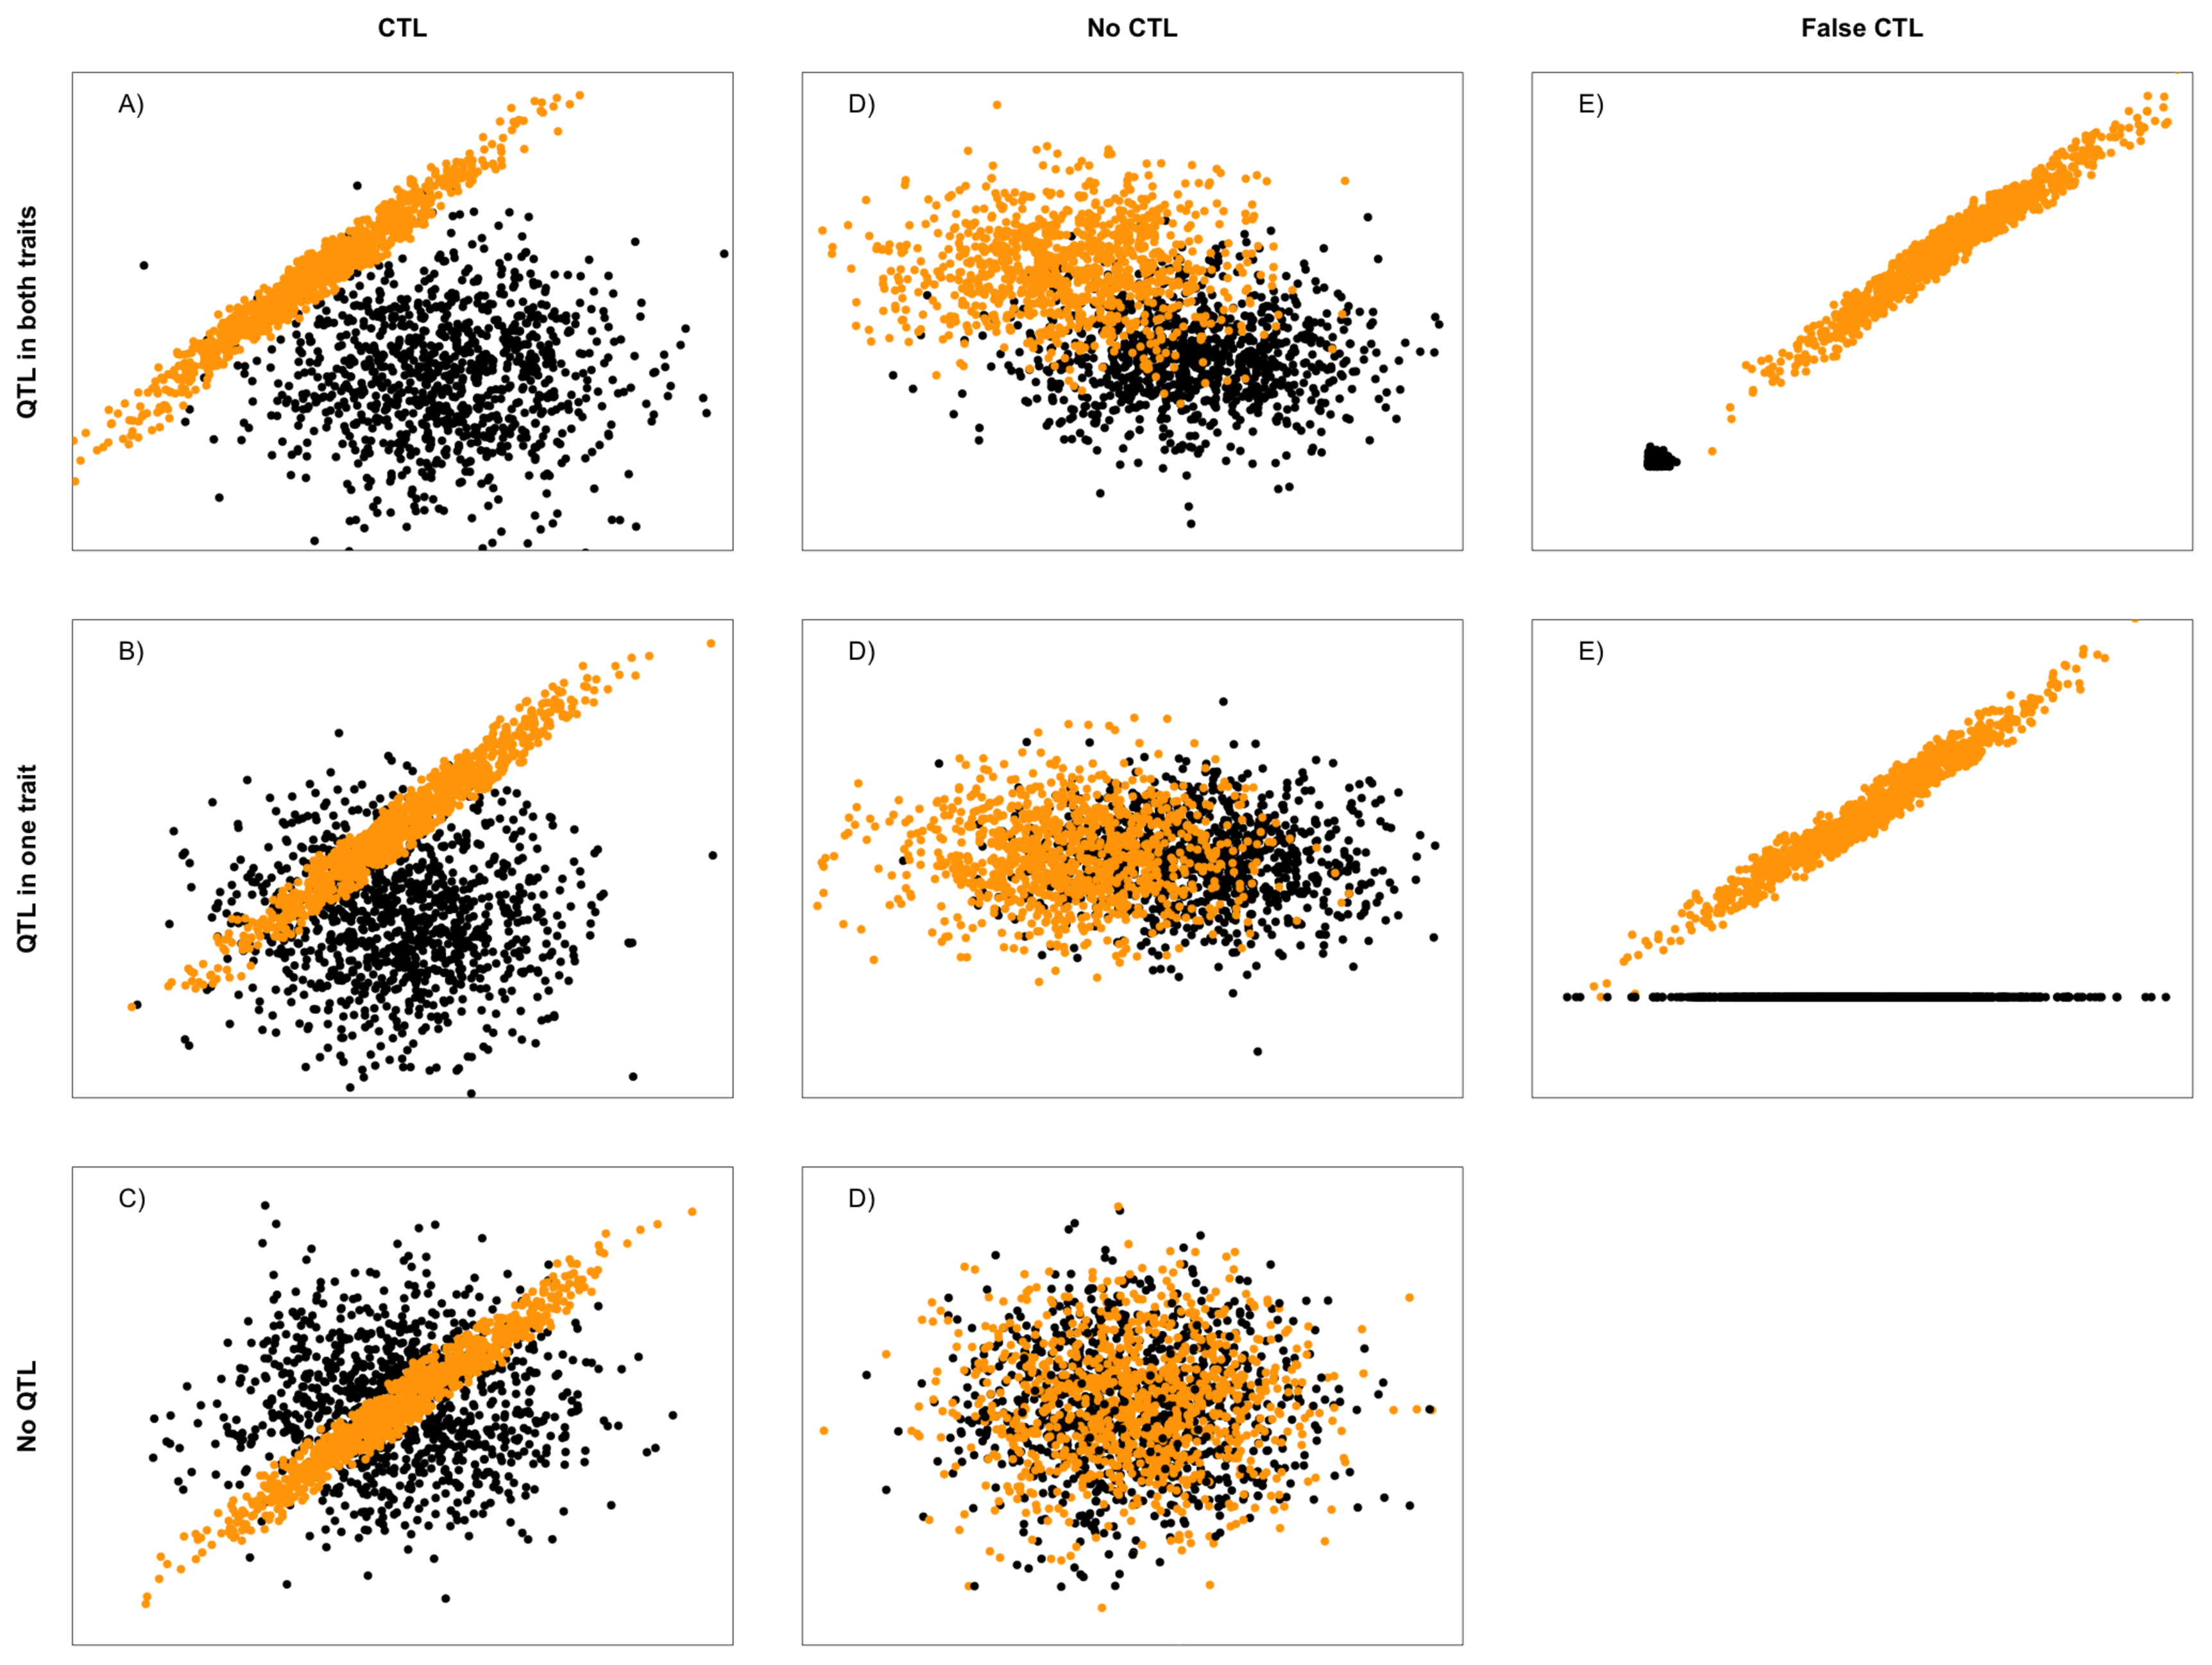
\includegraphics[width=0.9\textwidth]{eps/image_5_1.eps}
  \caption[CTLs.]{QTL and CTL analysis of two traits: a schematic of possible scenarios at a given marker. A trait can 
          have a QTL or no QTL at the given marker: there are four possible combinations in QTL analysis with two traits. 
          The trait pair can also have a CTL or no CTL and in the combined QTL and CTL analysis: the total number of possible 
          combinations is eight. Three additional scenarios refer to special cases when one trait or both traits are not 
          expressed in one genotype. For sake of simplicity it is assumed in this figure that there are two genotypes only, 
          e.g. as in a BC or RIL population. [We also ignore possible info on cis- and trans-mapping for the moment]}
          \label{fig:ctls}
\end{figure}

  \subsection{QTL and CTL analysis of two traits}
  
  To describe the possible relationships between QTL and CTL we generate the possible scenario's as in figure \ref{fig:ctls}.\\
  {\bf(A)} The two traits have a QTL and a CTL at the given marker (1 scenario). This example shows the extreme scenario when the traits are 
  well correlated in one genotype and entirely uncorrelated in the other. The locus affects both the mean and the correlation. They could 
  have a regulatory factor in common, the effect of which is detected in QTL and CTL analysis.\\
  {\bf(B)} The two traits have a CTL at the given marker, but only one trait has a QTL at that marker (2 scenarios).  The locus affects the 
  correlation, and the mean of one trait only. They could have a regulator in common in which case the latter trait is downstream of the other 
  trait: this can happen e.g. if the locus leads to functionally different transcripts at equal expression levels for the trait without QTL, 
  and this effect is propagated to the trait with (therefore) a QTL.\\
  {\bf(C)} The two traits have a CTL but no QTL at the given marker (1 scenario). This example shows the extreme scenario when the traits 
  are well correlated in one genotype and entirely uncorrelated in the other.  The locus affects the correlation only. They could have a 
  regulatory factor in common, the effect of which is detected in CTL analysis only: e.g. if the locus leads to co-regulated transcription 
  in one genotype only.\\
  {\bf(D)} The two traits have no CTL at the given marker  (4 scenarios).  The locus does not change the correlation, it change the mean 
  if one or both traits have a QTL. The example shows the extreme scenario when both traits have a QTL but are entirely uncorrelated: they 
  could be downstream of the same or a different factor at the given region.\\
  {\bf(E)} The two traits have a CTL at the given marker, but the trait values are at the noise level in one genotype for one or both 
  traits (3 scenarios). This expression at noise level for one trait could result from e.g. hybridization failure for one genotype. One 
  or both traits can have a possibly artificial QTL and the two traits have a possibly artificial CTL. The example shows the scenario 
  when only one trait has a QTL.

\section{Inference of hierarchical relationship between traits}
  \subsection{Using information of co-localized CTL and QTL}
  Observing a significant CTL between T1 and T2 means that there is a factor (e.g. genetic regulator) located underneath 
  the CTL peak influencing the correlation between T1 and T2. This information of shared genetic control, therefore, 
  indicates that T1 and T2 are involved in the same biological pathway \cite{Tesson:2010}.

  The absence of QTL in trait T1 and the presence of QTL in trait T2 indicate that T2 is downstream of T1 in the 
  hierarchical network. The reasoning is that the variation caused by a genetic factor in T2 (QTL) has not 
  propagated to T1 \cite{Jansen:2009}. The reserve situation can also happen: Presence of QTL in trait T1 and the 
  absence of QTL in trait T2 indicate that T2 is upstream of T1 in the hierarchical network.

  The presence of QTL in both traits X and Y further confirms that T1 and T2 are related in the same pathway, and it 
  even allows us to go from inferring hierarchical relationship to causality using methods such as conditional 
  correlation \cite{Schadt:2007, Li:2010}.

  It should be noted that the colocalized CTL information does not exclude the existence of intermediate factor(s) 
  e.g. Z,  between T1 and T2 in the pathway, although the relative strengthness of correlation provides us 
  information on the distance among them in the network, e.g. higher correlation can indicate a shorter distance 
  between T1 and T2 in the network.\\

  \subsection{Using information of co-localized CTLs}
  When the CTLxy of X and Y co-localizes with CTLxz of X and Z and CTLyz of Y and Z, these three traits are possibly 
  involved in the same network. The relative effect sizes of these CTLs can be used to infer the order of X, Y and Z
  in the hierarchical network. For example, when CTLxy and CTLyz are larger than CTLxz, we can conclude that they 
  follow the order of X-Y-Z in the network, i.e. Y is in between of X and Z.

  Additionally when a QTL shows two or more co-localizing CTL we discovered a set of possible downstream targets 
  for the QTL. Which, when sample sizes permit, can be further annotated using gene ontology \cite{GeneOntology:2000} or 
  untangled by using methods like hierarchical inference (this paper) or causal inference \cite{Schadt:2005, Li:2006} 
  to obtain en even more detailed view of genetic regulation within the set.

  \subsection{Visualizing CTL information}
  Information obtained by CTL mapping can be visualized in several different ways the author found the most accessible 
  representation is a user-customizable network view. User customization helps researchers to add their own and/or 
  literature information to a network allowing for a rich interpretation of the created network. Network generated from 
  CTL mapping can be visualized by software tools including Cytoscape \cite{Cytoscape:2010, Cytoscape:2003}.

  CTL information allows us to draw lines from traits via markers to other traits reconstructing the underlying genetic 
  wireing. To create hierarchical networks we transforming the significant CTLs into network edges. This is done by 
  using a user defined genome wide FDR and then only transforming significant trait-marker-trait interactions into a 
  .sif network file.

\section{Cell type specific eQTL mapping in human GAWA data}
\label{sec:cellspecificeqtl}

